\chapter{User Interface Design}

\section{Navigation Overview}

\section{Mockup screens}
In the following section there are some mockups of the application together with the explanation of all the feature reachable by the represented screen.

\subsection{Log In}
\begin{figure}[H]
	\centering
	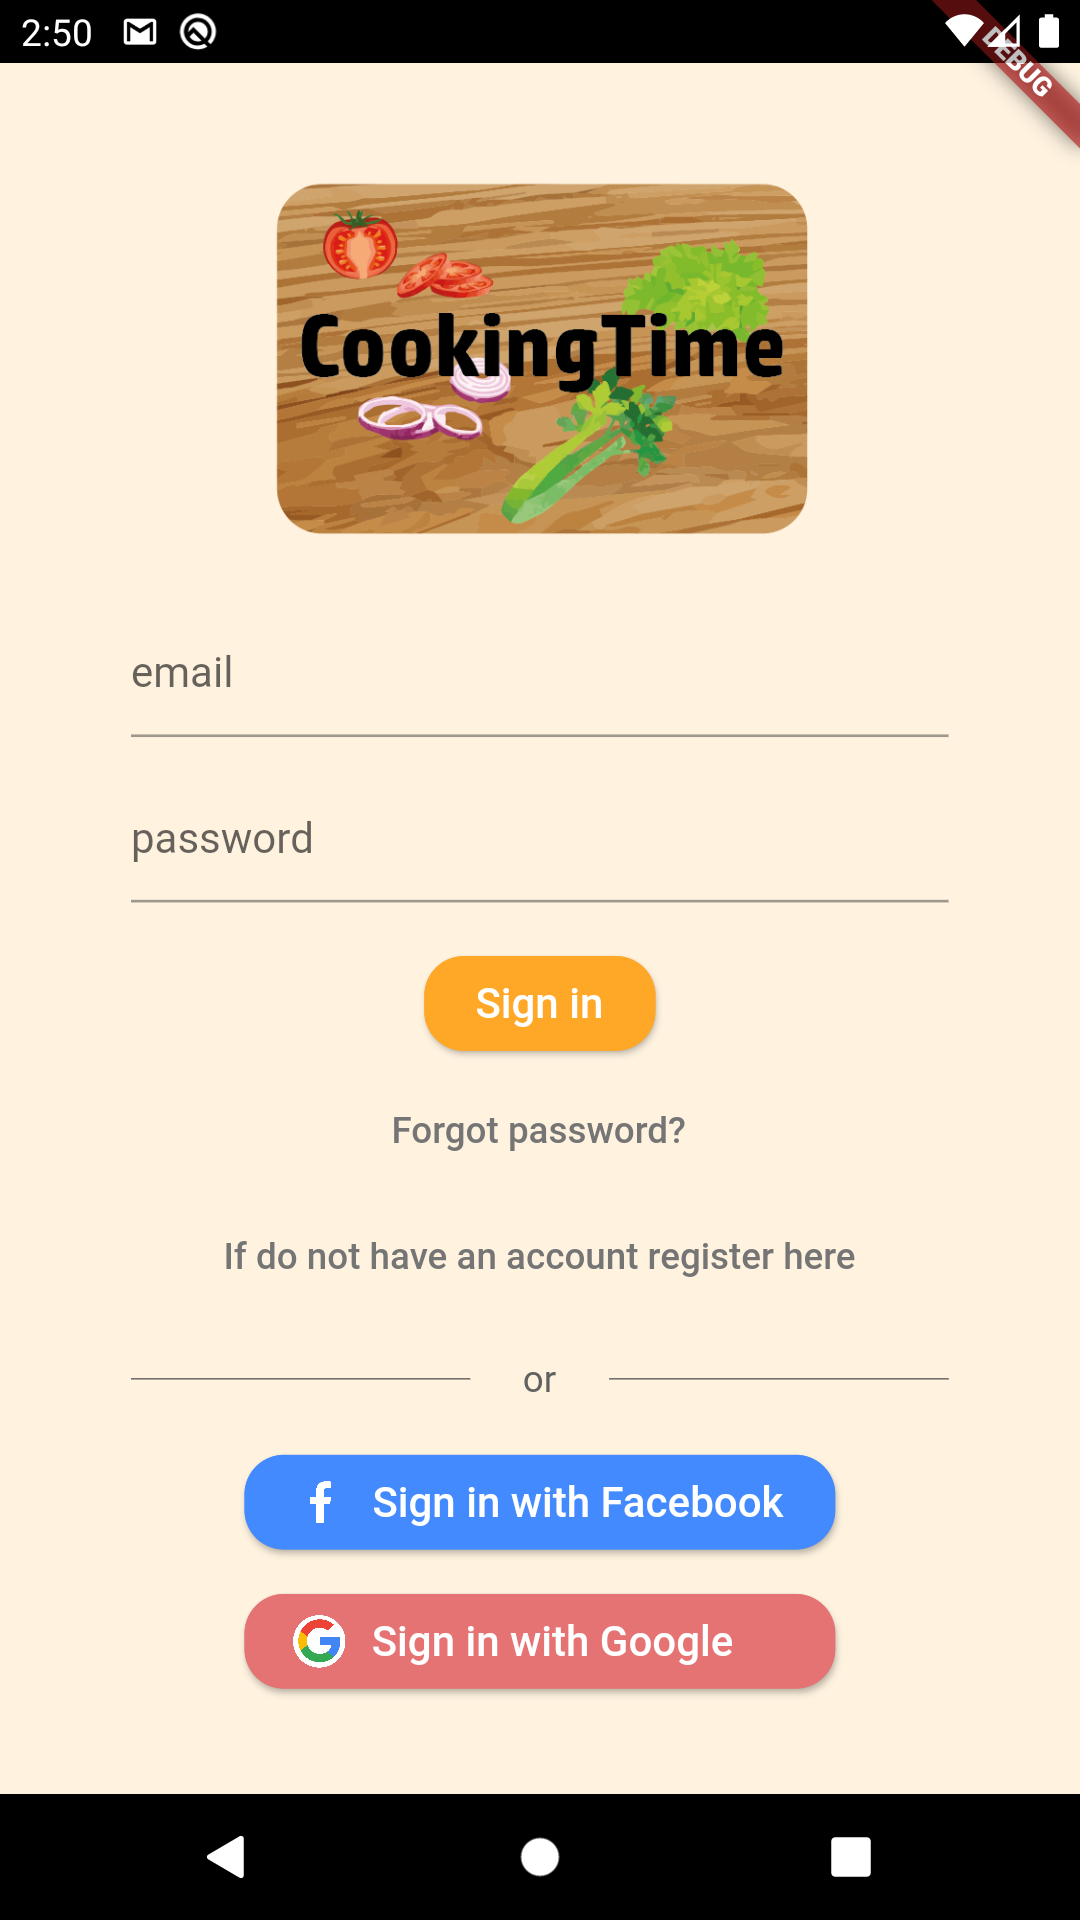
\includegraphics[width = .3\linewidth]{img/SignIn.png}
	\caption{Login Screen}
\end{figure}
This is the first screen which the user sees after the opening of the application, here he can login using his credential, moreover he can go to the registration page or the lost password page.
\subsection{Registration}
\begin{figure}[H]
	\centering
	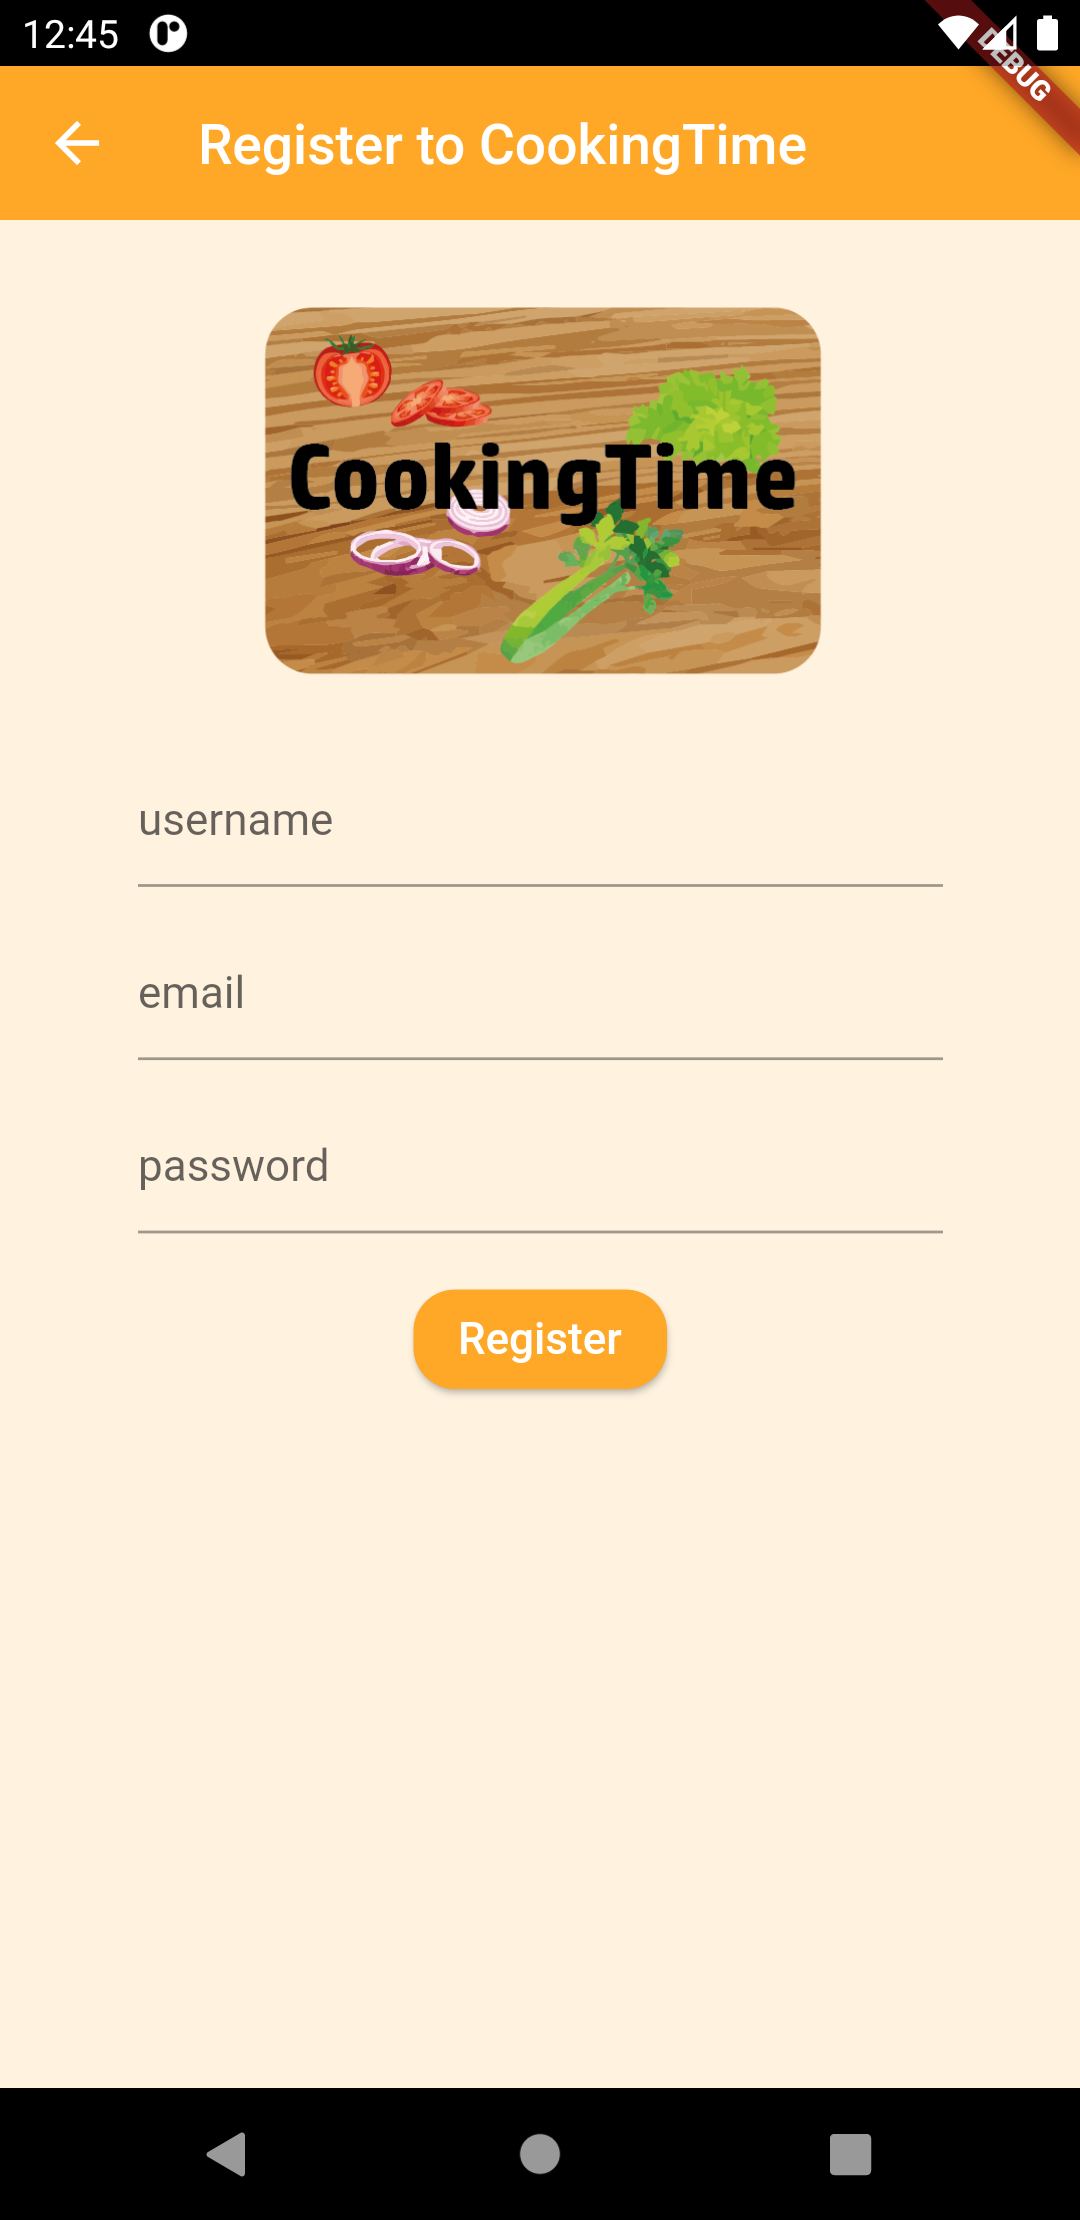
\includegraphics[width = .3\linewidth]{img/Registration.png}
	\caption{Resgistration Screen}
\end{figure}
This screen allows the user to register in the application providing a unsername, email and password.
\subsection{Password Reset}
\begin{figure}[H]
	\centering
	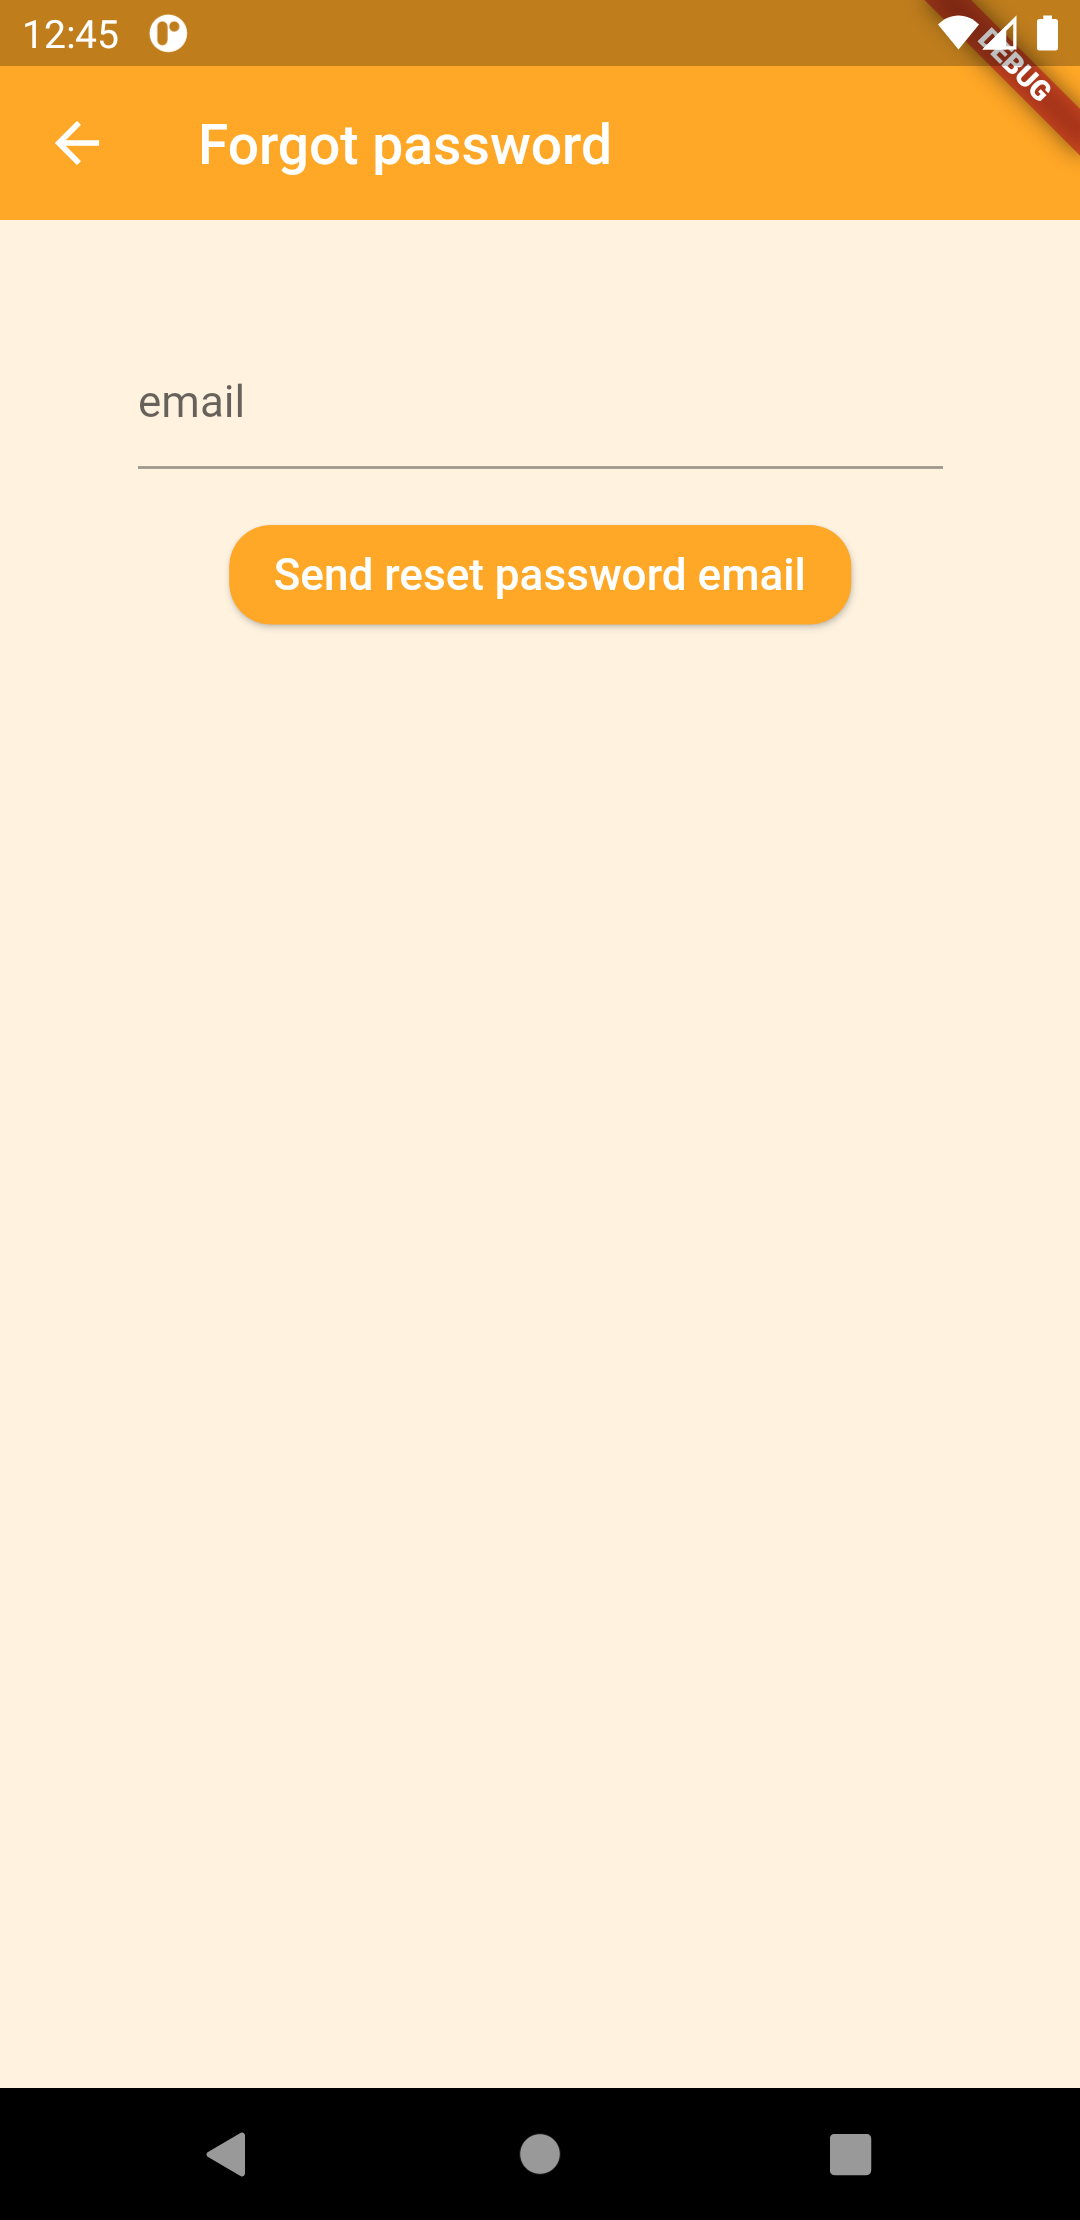
\includegraphics[width = .3\linewidth]{img/PasswordReset.png}
	\caption{Password Reset Screen}
\end{figure}
From this screen the user has the possibility to restore his lost password, providing the email by which he made the registration before.
\subsection{Home}
%TODO image
This is the main screen of the appliaction, from here the user is able to navigate to all the available screen and feature of the application. It retrieves the ten most recent uploaded recipes and if he keeps scrolling more recipes are shown.
\subsection{Recipe Description}
\begin{figure}
	\begin{minipage}{0.48\textwidth}
		\centering
		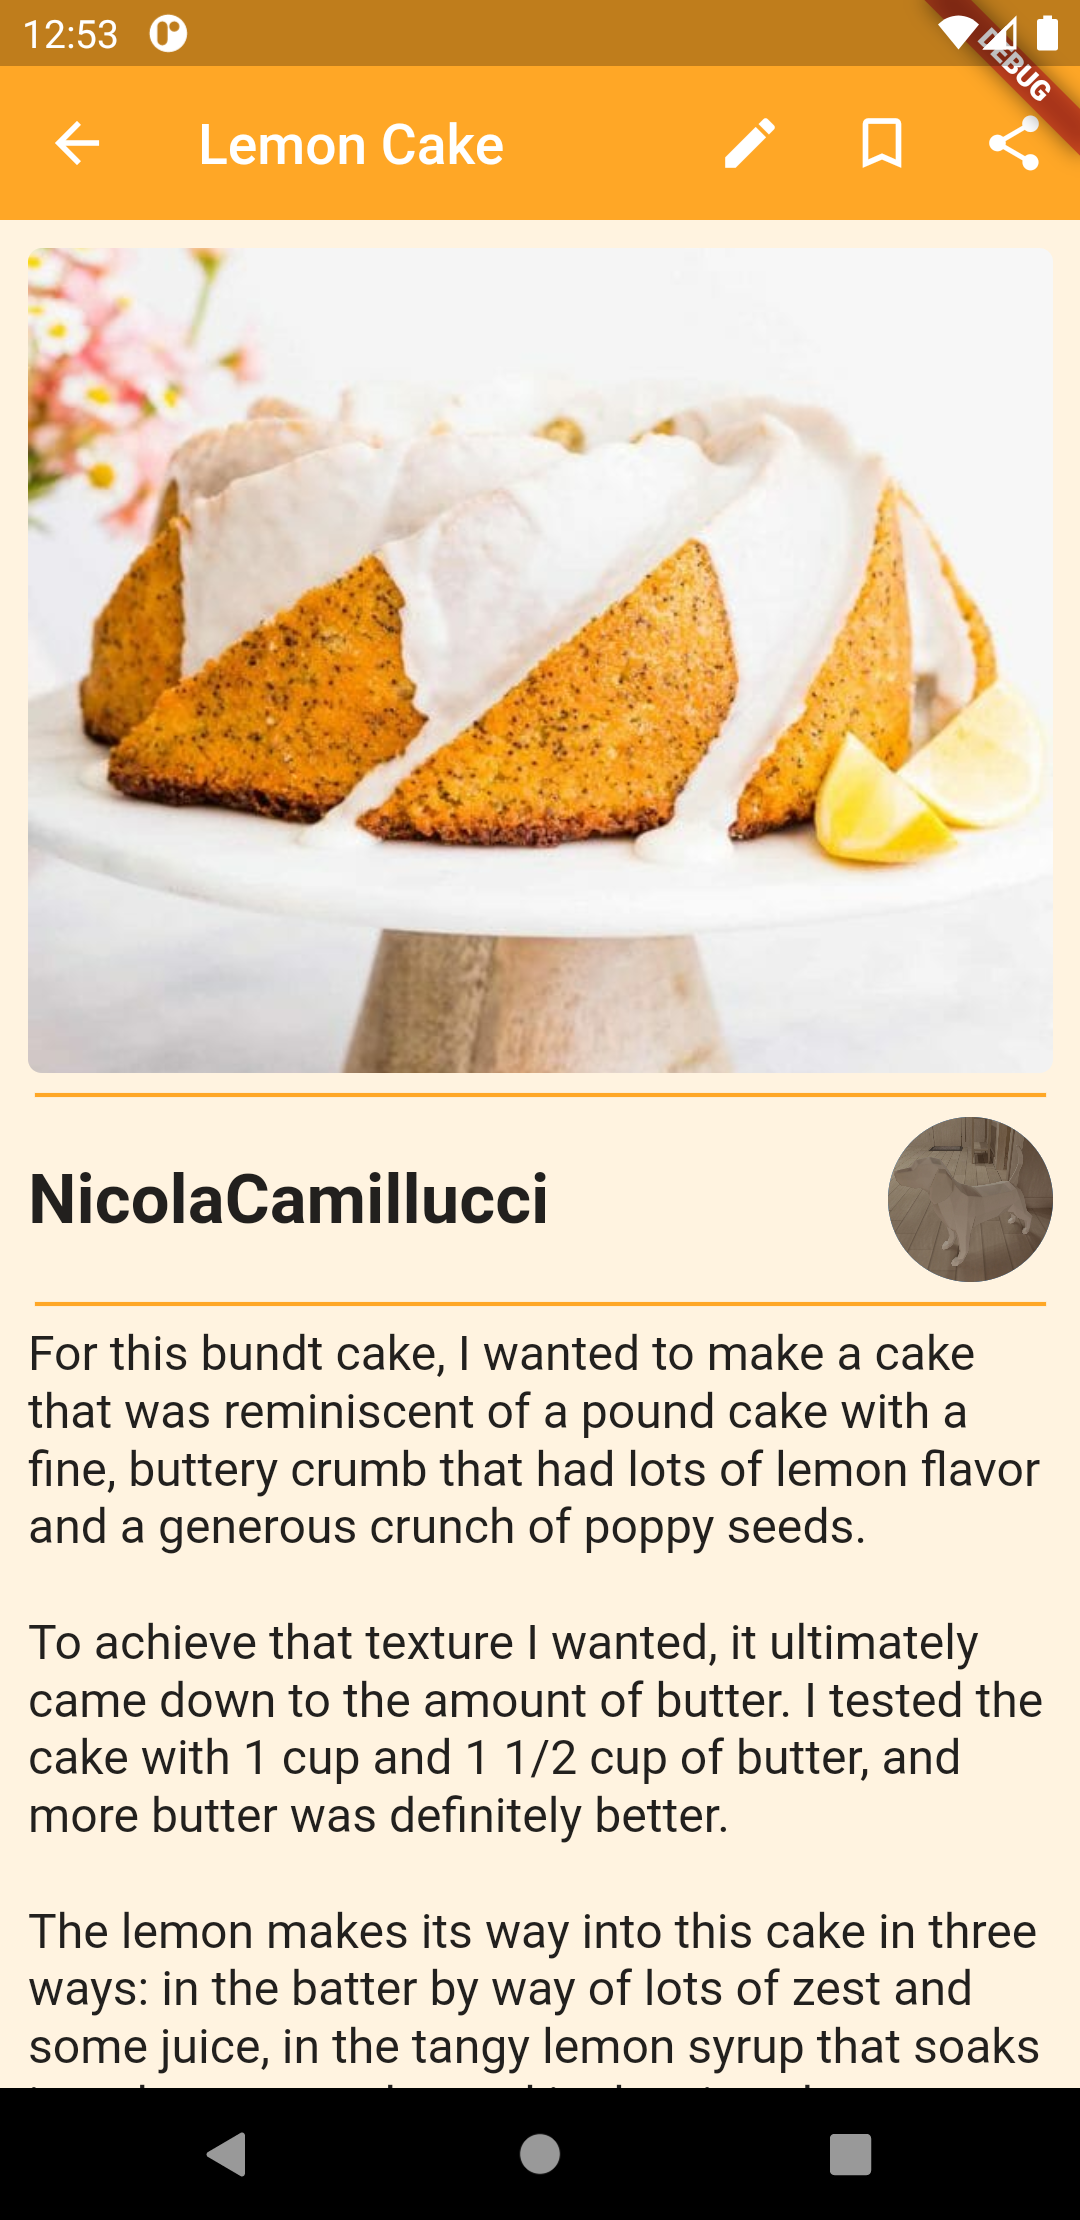
\includegraphics[width = .7\linewidth]{img/RecipeView.png}
		\caption{Recipe View 1 Screen}
	\end{minipage}\hfill
	\begin{minipage}{0.48\textwidth}
		\centering
		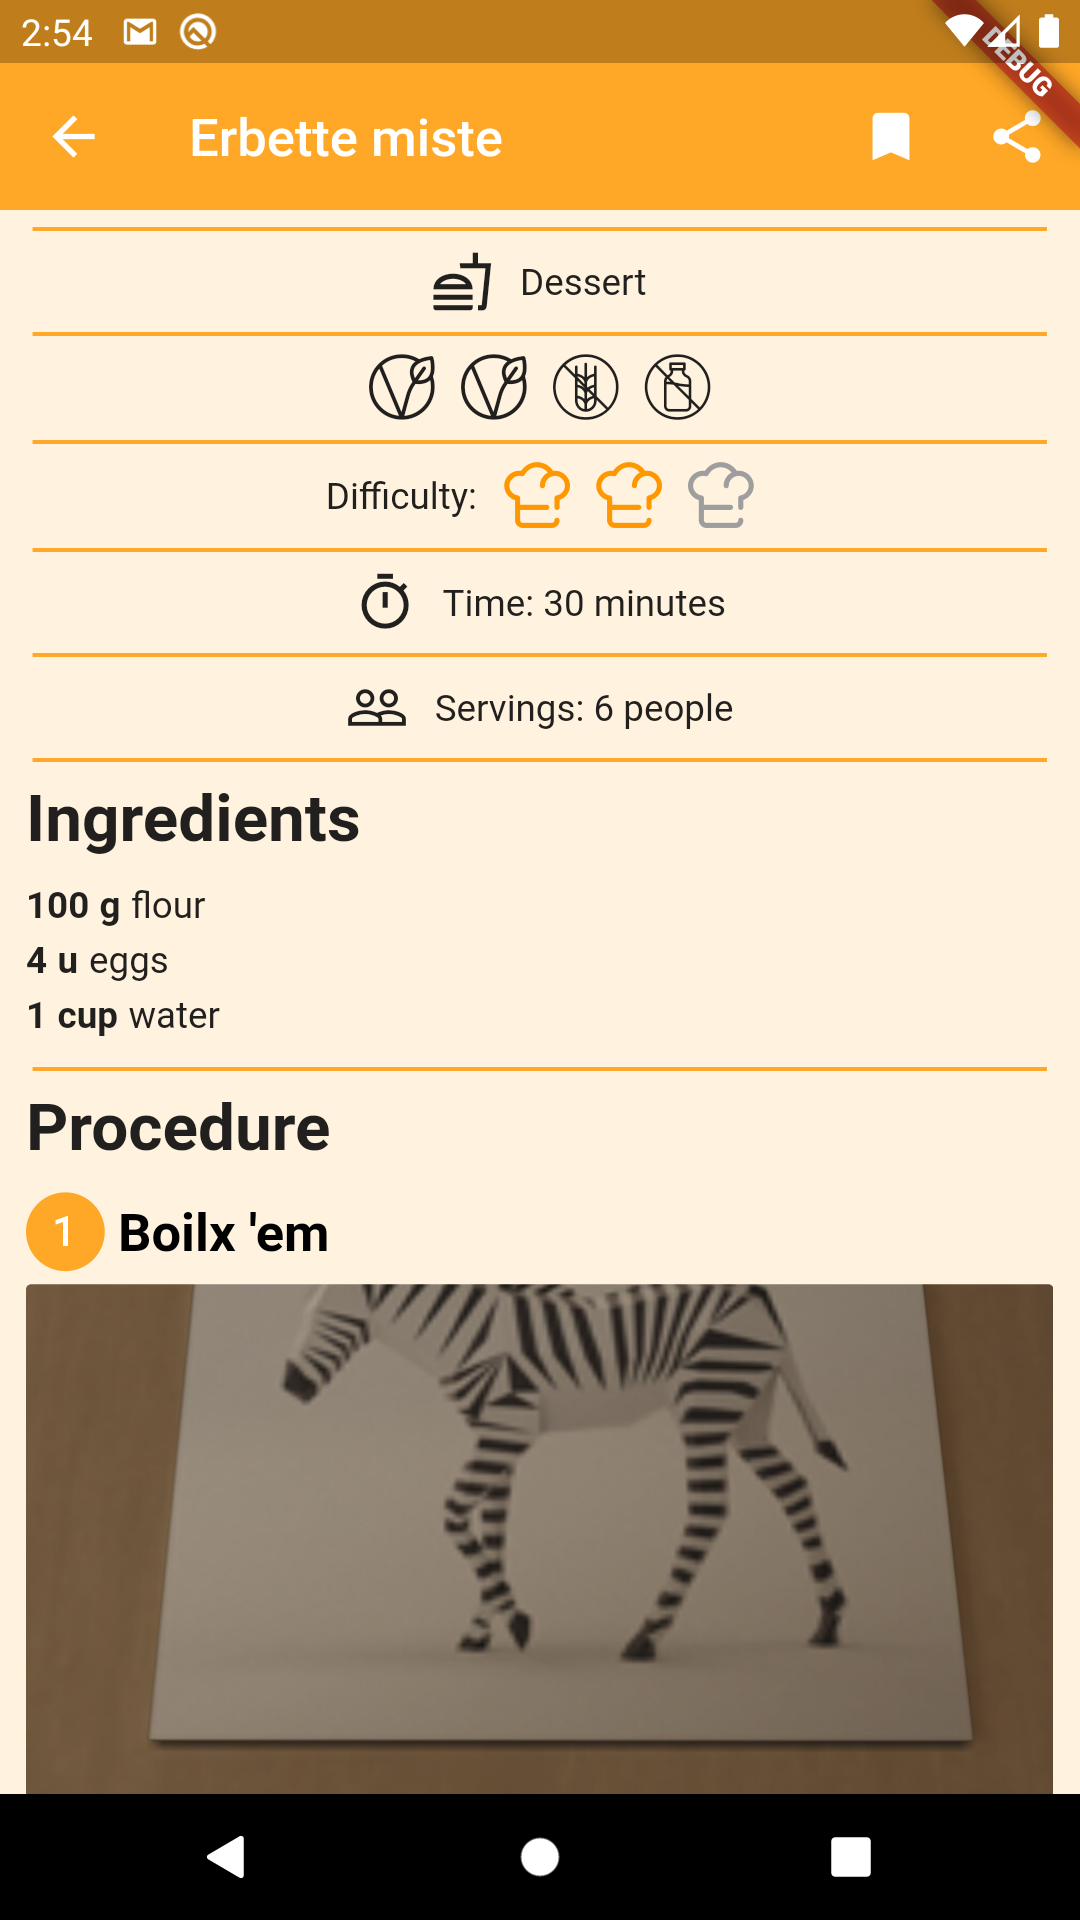
\includegraphics[width = .7\linewidth]{img/RecipeView_2.png}
		\caption{Recipe View 2 Screen}
	\end{minipage}
\end{figure}
This is the screen which appears after clicking on a recipe card, it shows the picture of the dish, the required ingredients and all the procedure to cook the recipe.
\subsection{Write a Recipe}
\begin{figure}[H]
	\begin{minipage}{0.31\textwidth}
		\centering
		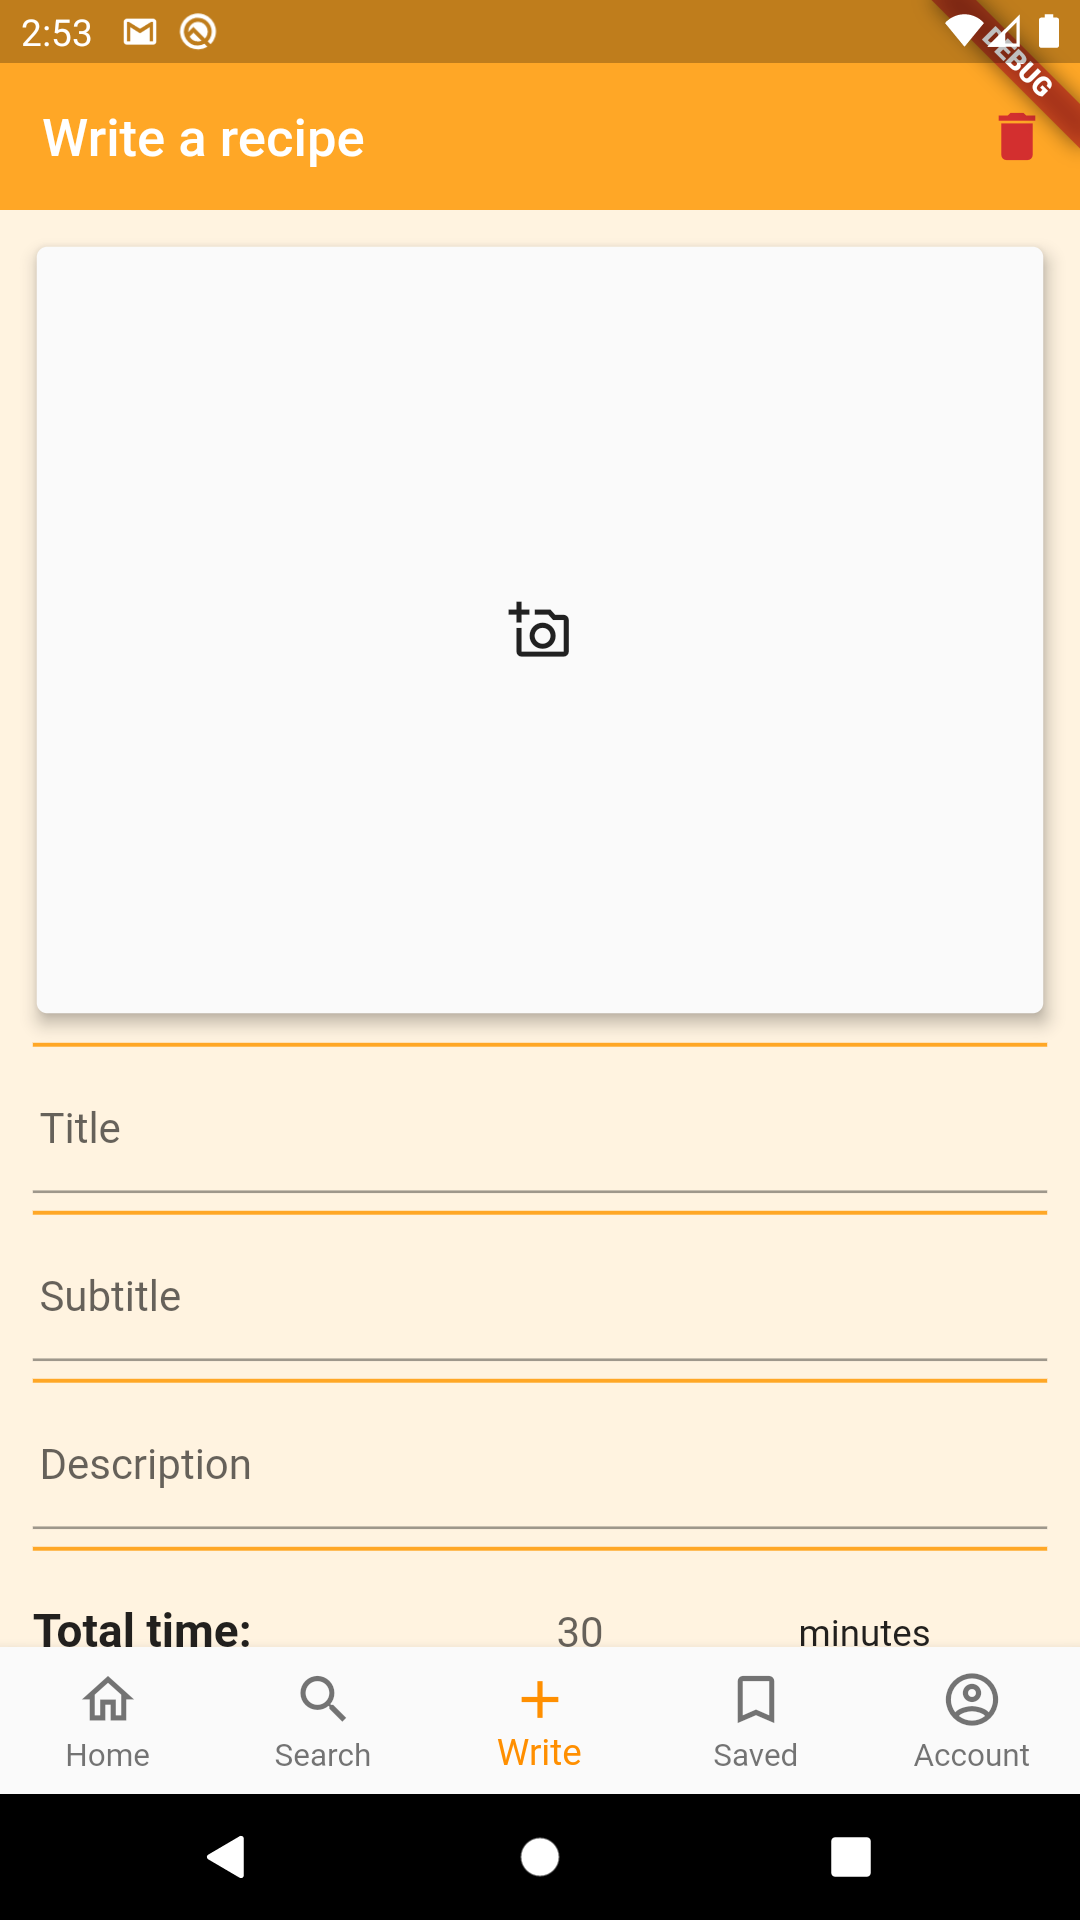
\includegraphics[width = .9\linewidth]{img/Write_1.png}
		\caption{Write Recipe 1 Screen}
	\end{minipage}\hfill
	\begin{minipage}{0.31\textwidth}
		\centering
		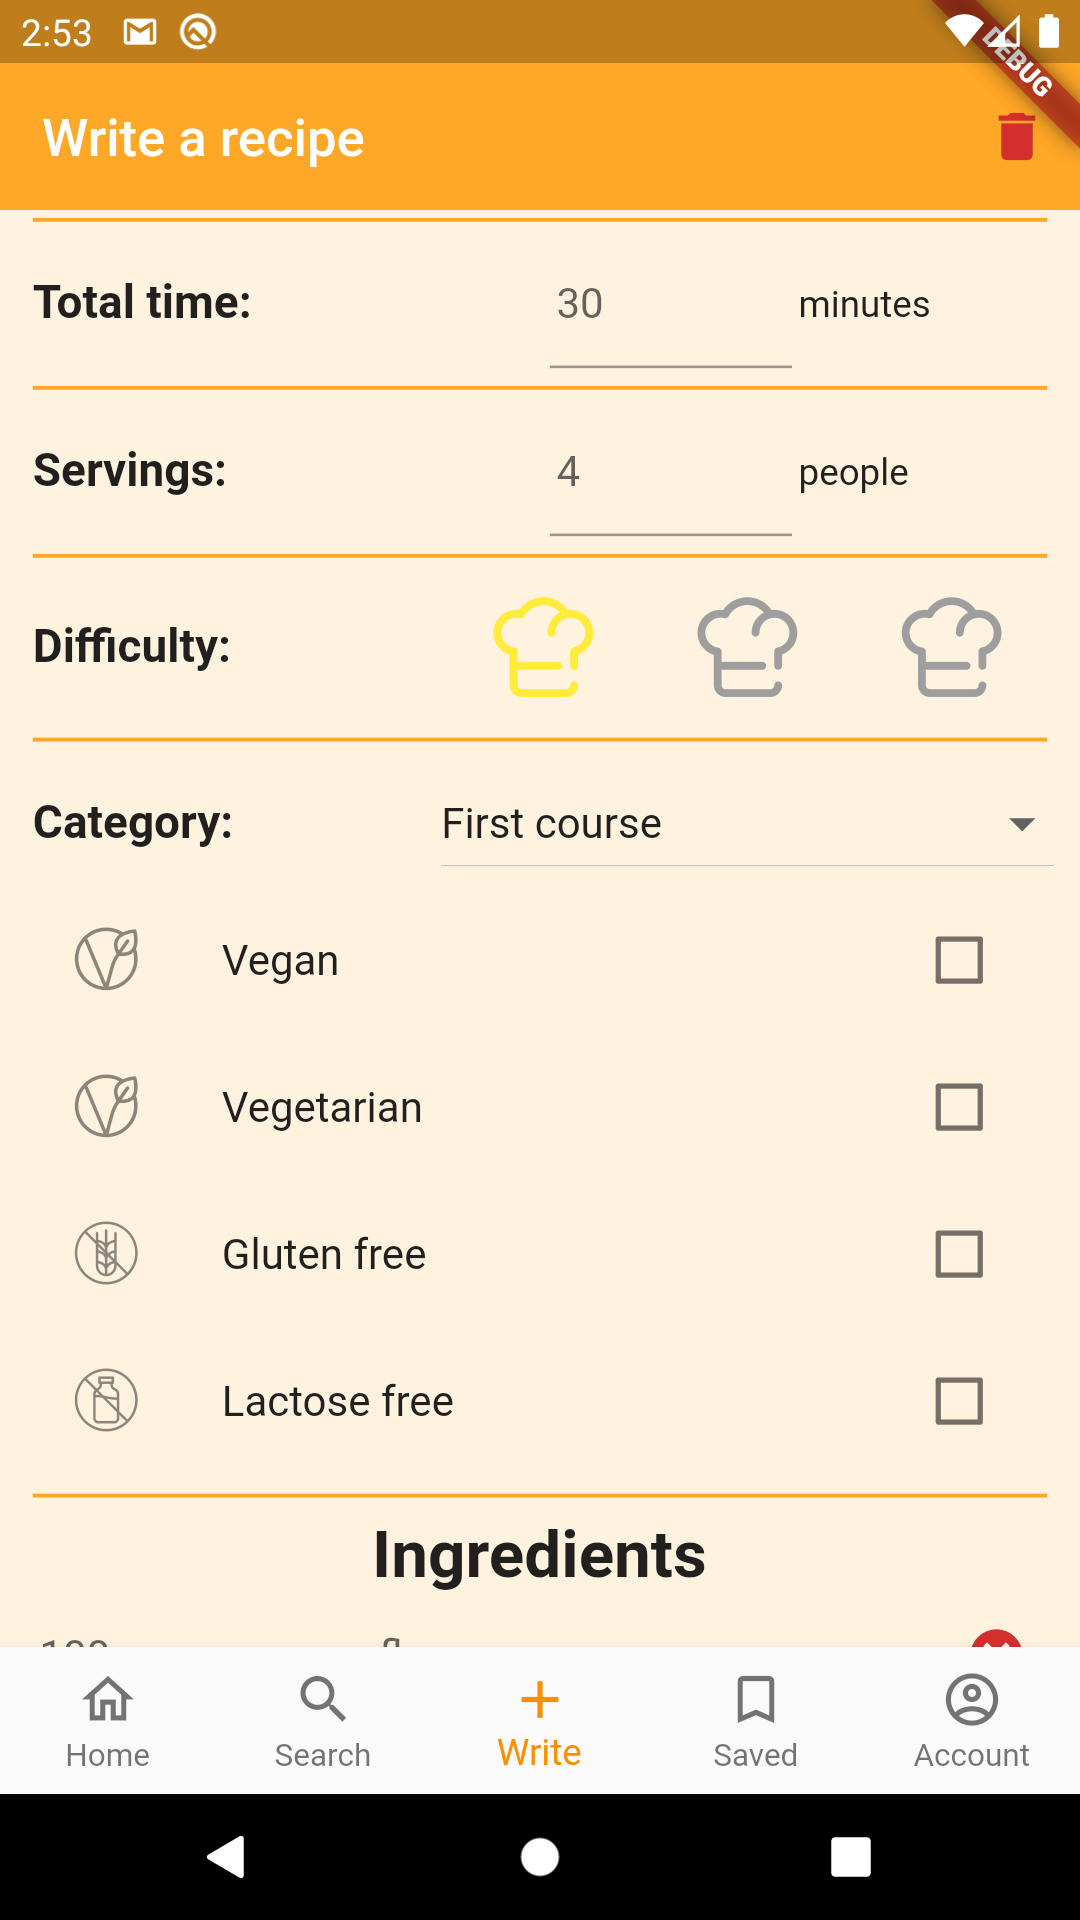
\includegraphics[width = .9\linewidth]{img/Write_2.png}
		\caption{Write Recipe 2 Screen}
	\end{minipage}\hfill
	\begin{minipage}{0.31\textwidth}
		\centering
		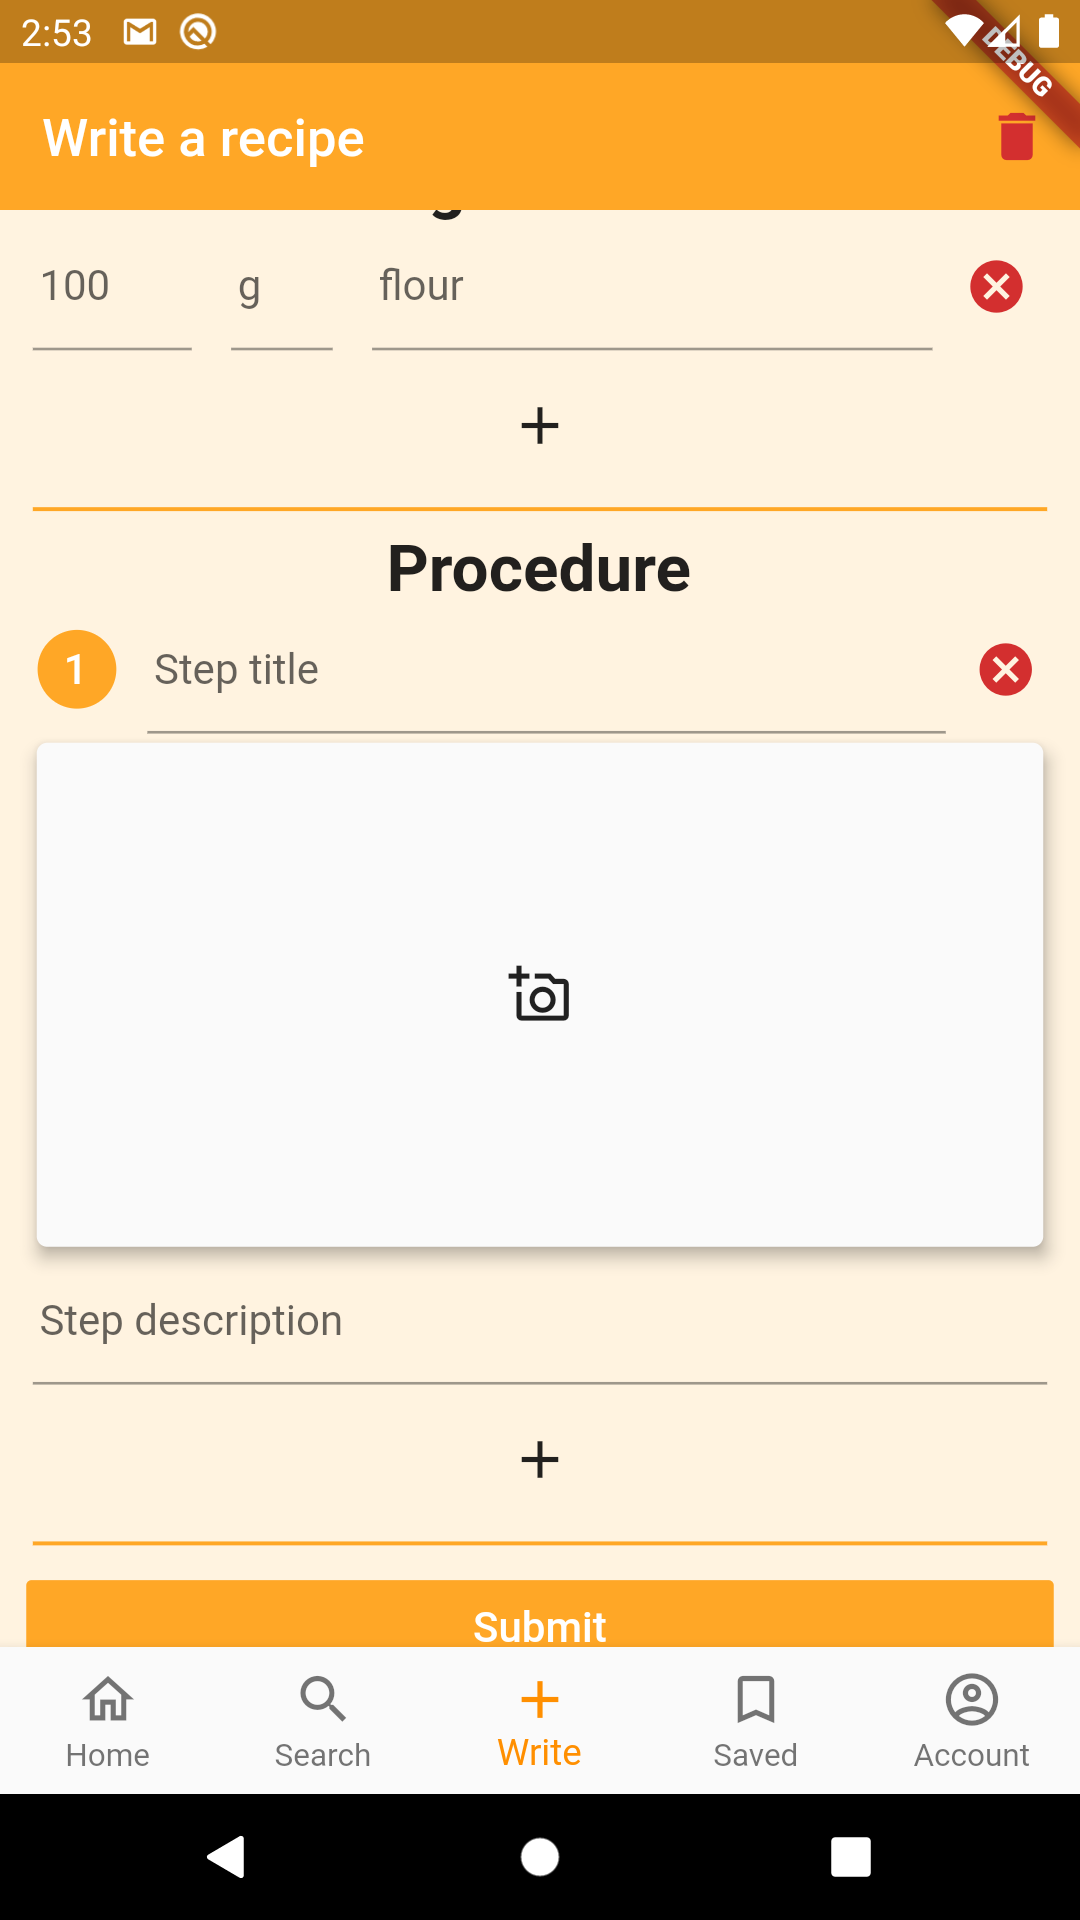
\includegraphics[width = .9\linewidth]{img/Write_3.png}
		\caption{Write Recipe 3 Screen}
	\end{minipage}
\end{figure}
This is the screen in order to insert a new recipe, it's reachable from the home page, here the user can provide the name of the recipe, the picture of the dish, some information especially the ingredients and procedure steps.
\subsection{Search Recipes}
\begin{figure}[H]
	\centering
	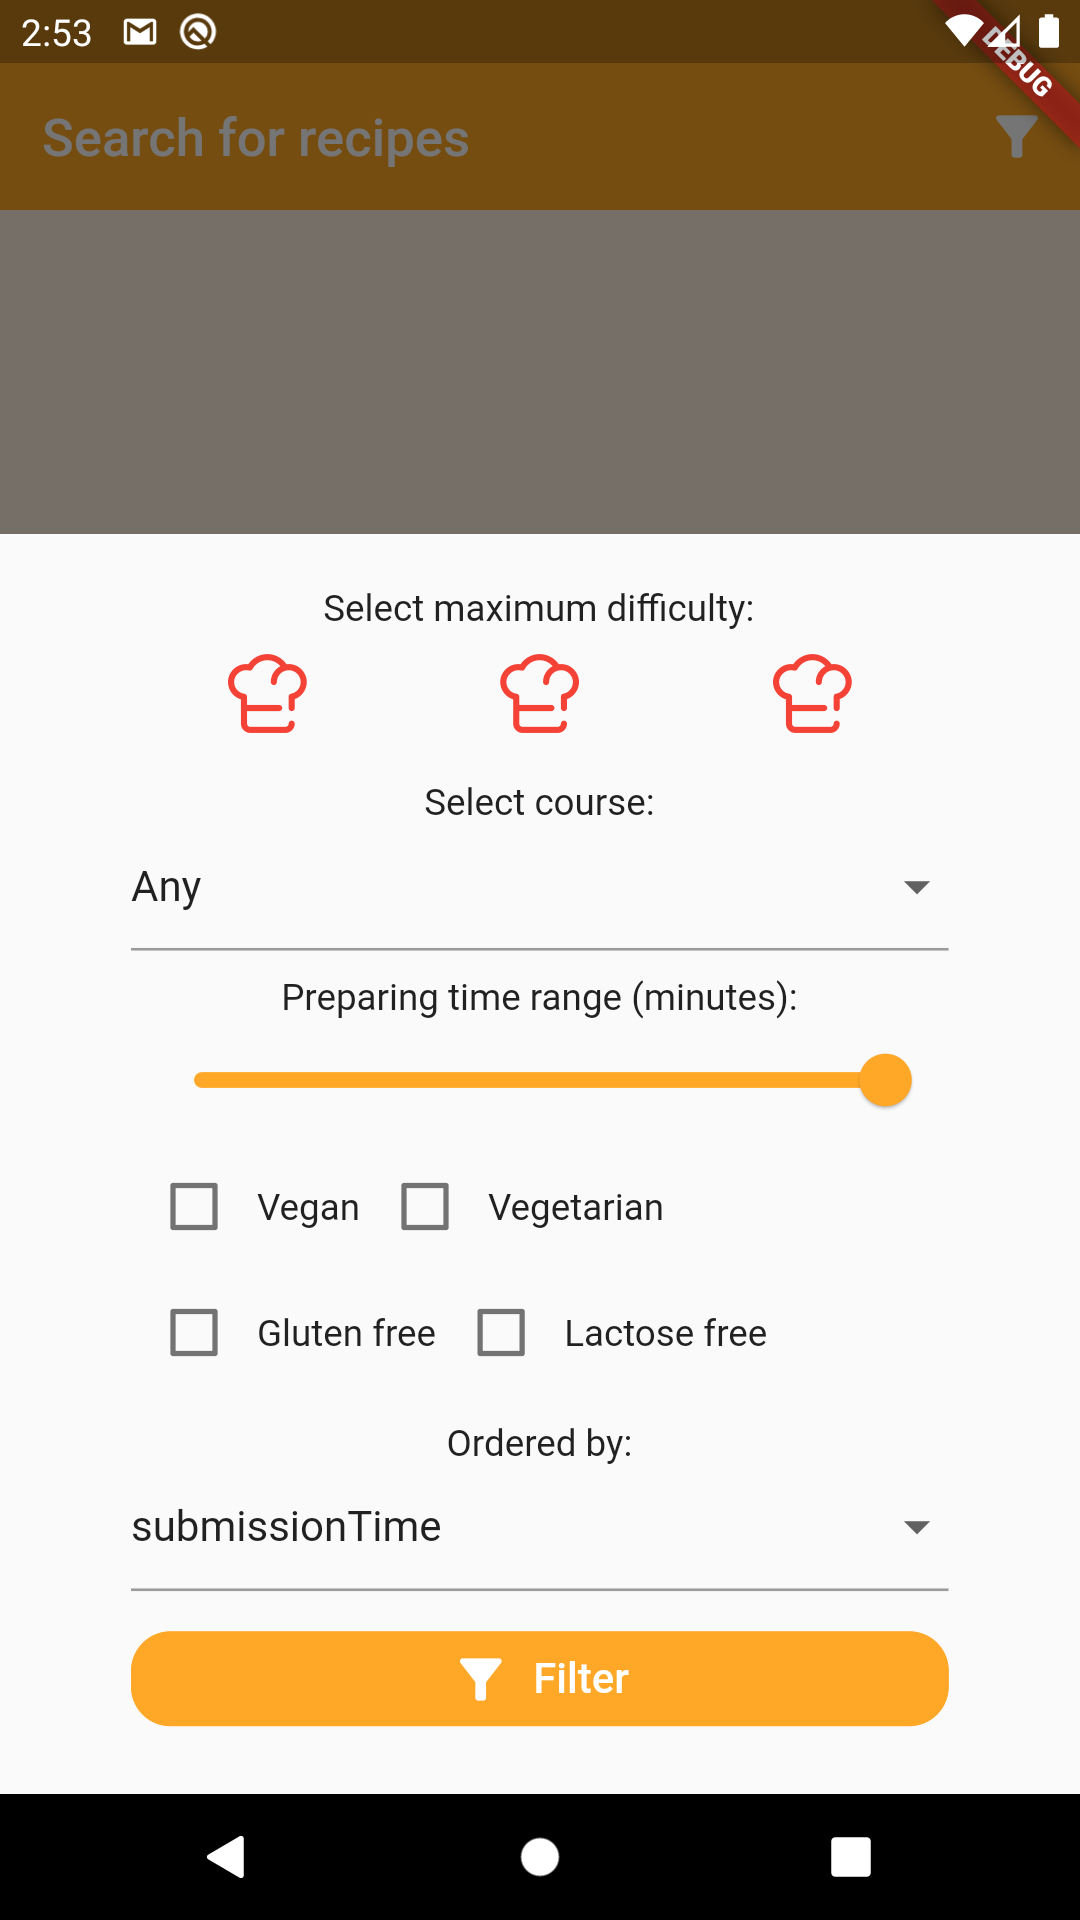
\includegraphics[width = .3\linewidth]{img/Filter.png}
	\caption{Search Recipe Screen}
\end{figure}
This screen, reachable from the home one, gives the possibility to filter the whole database of recipes according to some parameter like duration, difficulty, characteristics...
\subsection{Write a Review}
\begin{figure}[H]
	\centering
	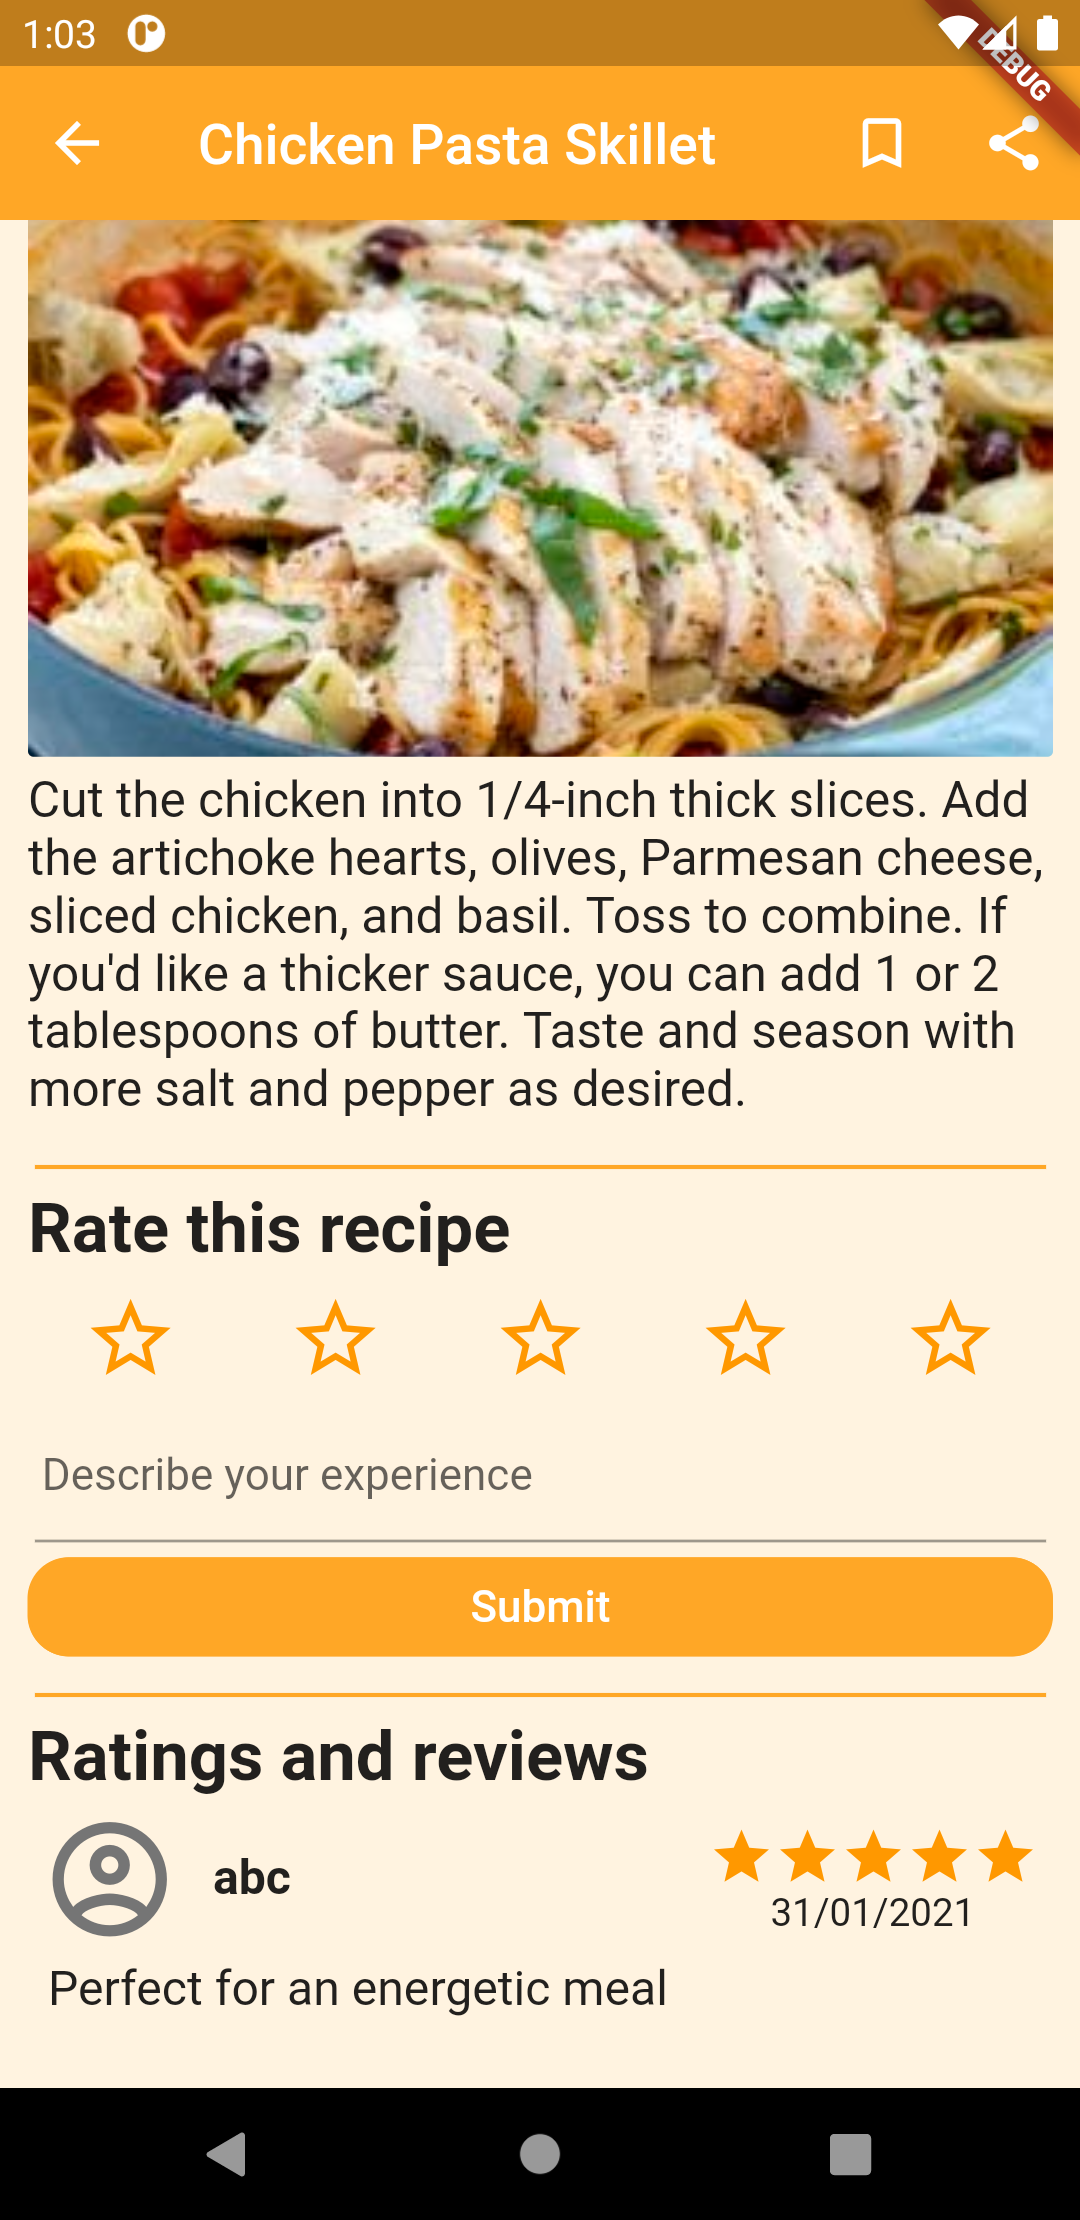
\includegraphics[width = .3\linewidth]{img/Review.png}
	\caption{Review Screen}
\end{figure}
This screen allows the user to create and rate a recipe made by another user.
\subsection{Saved Recipes}
\begin{figure}[H]
	\centering
	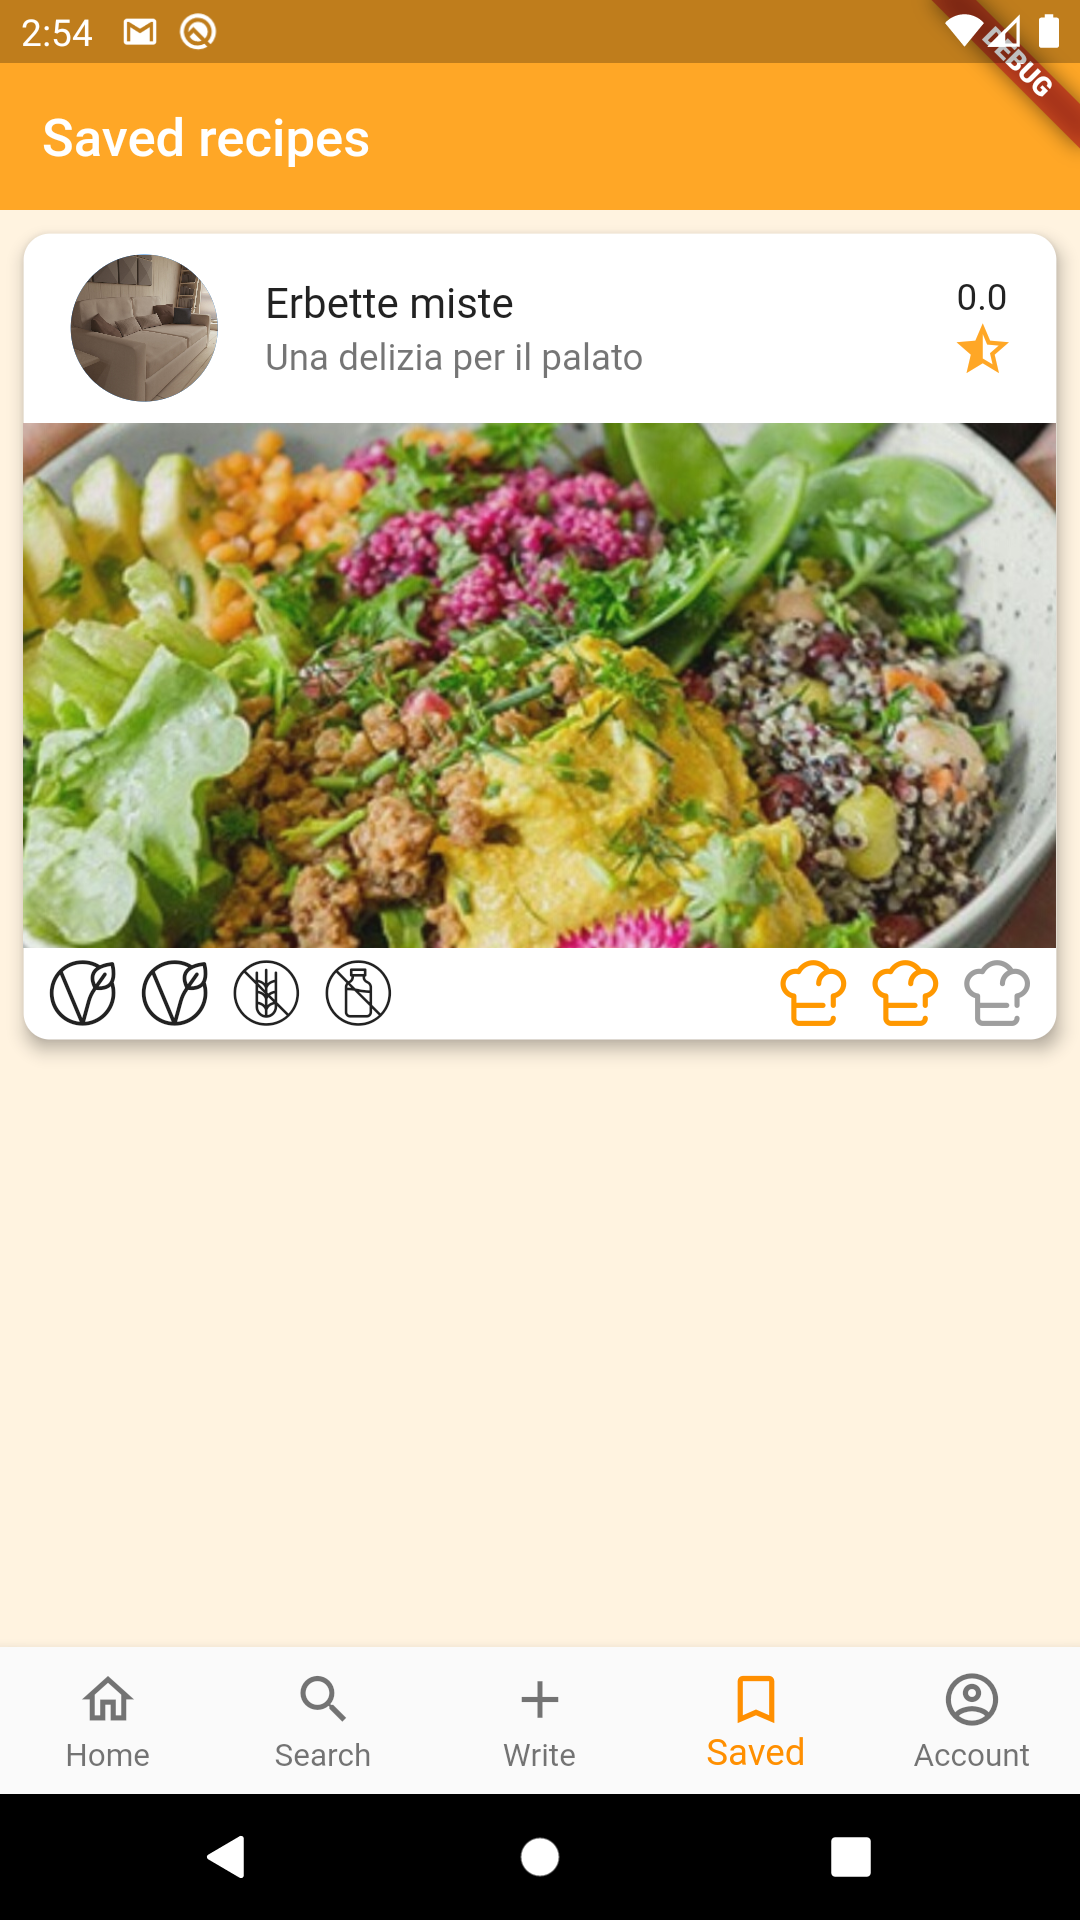
\includegraphics[width = .3\linewidth]{img/Saved.png}
	\caption{Saved Recipe Screen}
\end{figure}
This screen accesible from the home screen lists the reciped saved by the user.
\subsection{User Profile}
%TODO image
This screen shows the user profile statistics and the list of the user uploaded recipes.
\subsection{Settings}
%TODO image
This screen allows the user to modify his profile picture, username and the password (only if he is logged using the email).